\documentclass{article}
\usepackage{xcolor}
\usepackage{textcomp}
\usepackage{hyperref}
\usepackage{subfig}
\usepackage{subcaption}
\usepackage{graphicx}
\usepackage{wrapfig}
\usepackage{amsmath}
\usepackage[a4paper, margin=1in, footskip=0.25in]{geometry}

% relative path to images directory
% \graphicspath{ {./images/} }
\newcommand{\round}[1]{\ensuremath{\lfloor#1\rceil}}

% make captions of figures cursive
\DeclareCaptionFormat{custom}
{
    \textbf{#1#2}\textit{\small #3}
}
\captionsetup{format=custom}

\title{Research of Parameters in Strategies of the Iterated Continuous Prisoner's Dilemma}
\author{Adrian Hossner}
\date{ } % display no date

\begin{document}
\maketitle

\newpage
\tableofcontents
\newpage

\section*{Abstract}

\section{Introduction}

\begin{itemize}

	% Key idea:
	% Much uncertainty spread out because of (far-)right populists.
	% With insecurity comes random behaviour.
	% This simulations shows the difference of a random and a determined strategy.

	\item Interactions\\
		implication range is wide:\\
		from two persons in a relationship to countries in alliance\\
		from two impala's algrooming to zebras warning the herd about a lion \\
	% https://www.cell.com/trends/ecology-evolution/pdf/S0169-5347(00)88988-0.pdf

	\item Key hook:\\
		helping someone with possible cost -- cooperation\\
		being selfish but breaking trust -- defection\\

	\item Game Theory (optional, not needed for understanding)\\
		mathematical framework to investigate interactions\\

	\item model PD:\\
		single interaction\\
		already well analysed\\
		Nash found solution/equilibrium\\

	\item Iterated:\\
		more interesting, insightful\\
		strategies\\

	\item non-suited variants:\\
		Axelrod's Tournament\\
		Evolution\\

	\item continuous:\\
		more complex, accurate\\

	\item parameters:\\
		determines behaviour\\
		create surface\\
		the part that has not been experimented\\

	\item overall and difference:\\
		overall: wealth of population\\
		difference: competence between individuals\\

\end{itemize}

\section{Theoretical Foundations}

To grasp the game-theoretical approach pursued in this thesis, it is necessary to first understand the underlying key concepts. 
The most important ones being the Prisoner's Dilemma (PD) (2.1), the introduction of iterations as an extension (2.2) and the approach of submitting continuous values (2.3).
Furthermore, relevant information of published researches are provided as it seems helpful (2.5).

\subsection{Prisoner's Dilemma}
		
The Prisoner's Dilemma (PD) is a famous model in Game Theory. 
It was invented by Merrill Flood and Melvin Dresher in 1950. 
To understand the dilemma, a proper context has to be established.\\
Two persons are arrested and sued for having committed a crime jointly.
There is yet, however, insufficient evidence to imprison the two suspects.
Despite not having enough prove, the police utilises one of its methods.
They interrogate them separately without giving them a chance to coordinate beforehand.
The convicts receive two options.
On one hand, they can confess that the other suspect was involved in the crime. 
On the other hand, they have the right to remain silent.
Naturally, the police rewards the act of revealing the accomplice's delinquency over exercising the right of solidarity.
In case mutual trust and thus no confession took place, the twain separately receives an imprisonment of three years.
If both confess, either obtains five years in prison.
Nevertheless, by taking this course of action, this outcome is not the only existing.
If one chooses to confess while the other remains silent, the informer is released, whereas the betrayed must devote ten years in prison.
Remaining silent is considered as cooperation.
Whereby defection is the opposite, meaning breaking confidence and therefore state.
The following matrix visualises the pay-offs in this game in a comprehensive way:

% specific pay-off matrix
\begin{center}
\begin{tabular}{ c|c|c }
   & C & D \\ 
   \hline
 C & 3, 3 & 0, 10\\  
   \hline
 D & 10, 0 & 5, 5
\end{tabular}
\end{center}

\noindent
C represents cooperation and D corresponds to defection. 
The dilemma consists of the following.\\
The act of confessing appears alluring since there is a chance of eluding imprisonment.
Nonetheless, it is possible to receive five years in prison depending on the confederate's decision.
If the second criminal also confesses, both get five years in prison. 
This is the most inferior outcome for both which could have been avoided as either would have stayed silent.\\
John Nash, a mathematician which made great contributions in Game Theory, has proved the most reasonable course of action to be confessing.
The Nash-equilibrium is introduced. 
It defines a stable state in which both would not reconsider their own judgement although each of them would be aware of the other's decision.\\
This game composes a one-time interaction excellently in a mathematical and analytical perspective. 
The entitlement of the variables derives form the pay-off they suggest.\\
$T$: Temptation,
$R$: Reward,
$P$: Punishment,
$S$: Sucker's pay-off\\
The pay-offs in the matrix can be altered as long as these inequalities stay valid.
% \url{https://www.investopedia.com/terms/n/nash-equilibrium.asp}

% general pay-off matrix
\begin{center}
\begin{tabular}{ c|c|c }
   & C & D \\ 
   \hline
 C & R, R & S, T\\  
   \hline
 D & T, S & P, P
\end{tabular}
\end{center}

$$T > R > P > S$$

\subsection{Iterated}
		
The Iterated Prisoner's Dilemma (IPD) is a game which extends the PD. 
As the name suggests, the PD is played a number of times sequentially. 
To refer to the number of rounds played, $n$ is used as the denotation. 
The gained pay-offs accumulated over the last $n-i$ rounds are summed where $i$ represents the current round.
A strategy is an autonomous player which has its own behaviour.
Such a strategy has the whole history of the previous PDs at hand to generate the decision for the next round.
These decisions are calculated using conditions and probabilities that will be applied on the given data.
In this, and in the following variants, the analogy to the real world is changed.
Maximising one owns points is preferred.
Since a strategy strives to gain as many points as possible, the pay-off matrix must be altered accordingly.\\

\begin{center}
\begin{tabular}{ c|c|c }
   & C & D \\ 
   \hline
 C & 5, 5 & 10, 0\\  
   \hline
 D & 0, 10 & 3, 3
\end{tabular}
\end{center}

And to generalise this pay-off matrix as well, the numbers can be replaced with variables.
The concept is used for $T$, $R$, $P$, and $S$, provided that the four inequalities are satisfied.

\begin{center}
\begin{tabular}{ c|c|c }
   & C & D \\ 
   \hline
 C & R, R & S, T\\  
   \hline
 D & T, S & P, P
\end{tabular}
\end{center}

\begin{equation}
T < R < P < S\\
\end{equation}
\begin{equation}\label{AvGrPa}
2R > T + S
\end{equation}

Inequality \eqref{AvGrPa} is necessary to avoid receiving greater pay-offs by alternating cooperation and defection.\\
The Nash-equilibrium in the IPD differs from the that in the PD.
This implies that mutual cooperation yields long-term benefits.
Playing cooperation increases trust whereas defection allows exploitation.
Maximum pay-off during all the games is achieved only by consistent exploitation ($n \cdot T$).
Since persistent defection leads to mutual defection as a response, the practical attainment of the maximum points is severely limited.
To conclude, both strategies benefit the most with mutual cooperation.\\
A problem arises in the last round.
Since cooperation is only played to conserve trust, the reasonable action in the last round is to defect as trust has no use beyond the game.
If both strategies act rational, mutual defection will be played in the last round.
And because both are aware of this fact, there is no logical reason to cooperate the second last round.
This will end up in an inductive defection behaviour for both strategies the whole game.
So, to prevent constant mutual defection, the number of rounds played is an information that needs to be hidden from both strategies.
As a consequence of that, $n$ is a random number whose limits can be defined.\\
This extension of the PD allows to simulate a relationship of two individuals.

\subsection{Continuous}

In this variant, strategies are not limited to either cooperate or defect; instead, they can chose any level of cooperation between 0 and 1.
It is thus named Iterated Continuous Prisoner's Dilemma (ICPD)
This cooperation level, called investment or contribution, ranges from zero (defect) to one (cooperate).
The continuous form offers enhanced precision and mathematical applicability.\\
% One would suspect a very similar pay-off system to the iterated variant.
% In the discrete version, it looked like this:
%
% \begin{center}
% \begin{tabular}{ c c }
% Pay-off Player A & Pay-off Player B\\
% \begin{tabular}{ c|c|c }
%    & $C_A$ & $D_A$ \\ 
%    \hline
%  $C_B$ & 3 & 5\\  
%    \hline
%  $D_B$ & 0 & 1
% \end{tabular}
% &
% \begin{tabular}{ c|c|c }
%    & $C_A$ & $D_A$ \\ 
%    \hline
%  $C_B$ & 3 & 0\\  
%    \hline
%  $D_B$ & 5 & 1
% \end{tabular}
% \end{tabular}
% \end{center}

Two main approaches will be presented and evaluated for practicality in this thesis.
First, an intuitive extension of the iterated form. And second, a way that simplifies mathematically analysability.\\
A similar concept can be used to calculate the pay-offs given the investments of both strategies.
This concept is referring to a matrix-like pay-off system.
To include continuous values, a mathematical procedure is applied to the discrete version of the matrix, namely bilinear interpolation.
This will establish a field that can be represented by colour grades, a heat map.
Please see Figure \ref{fig:heatmaps}.
The equation used to calculate this heat map can be found in the Appendix.

\begin{figure}[h]
	\centering
	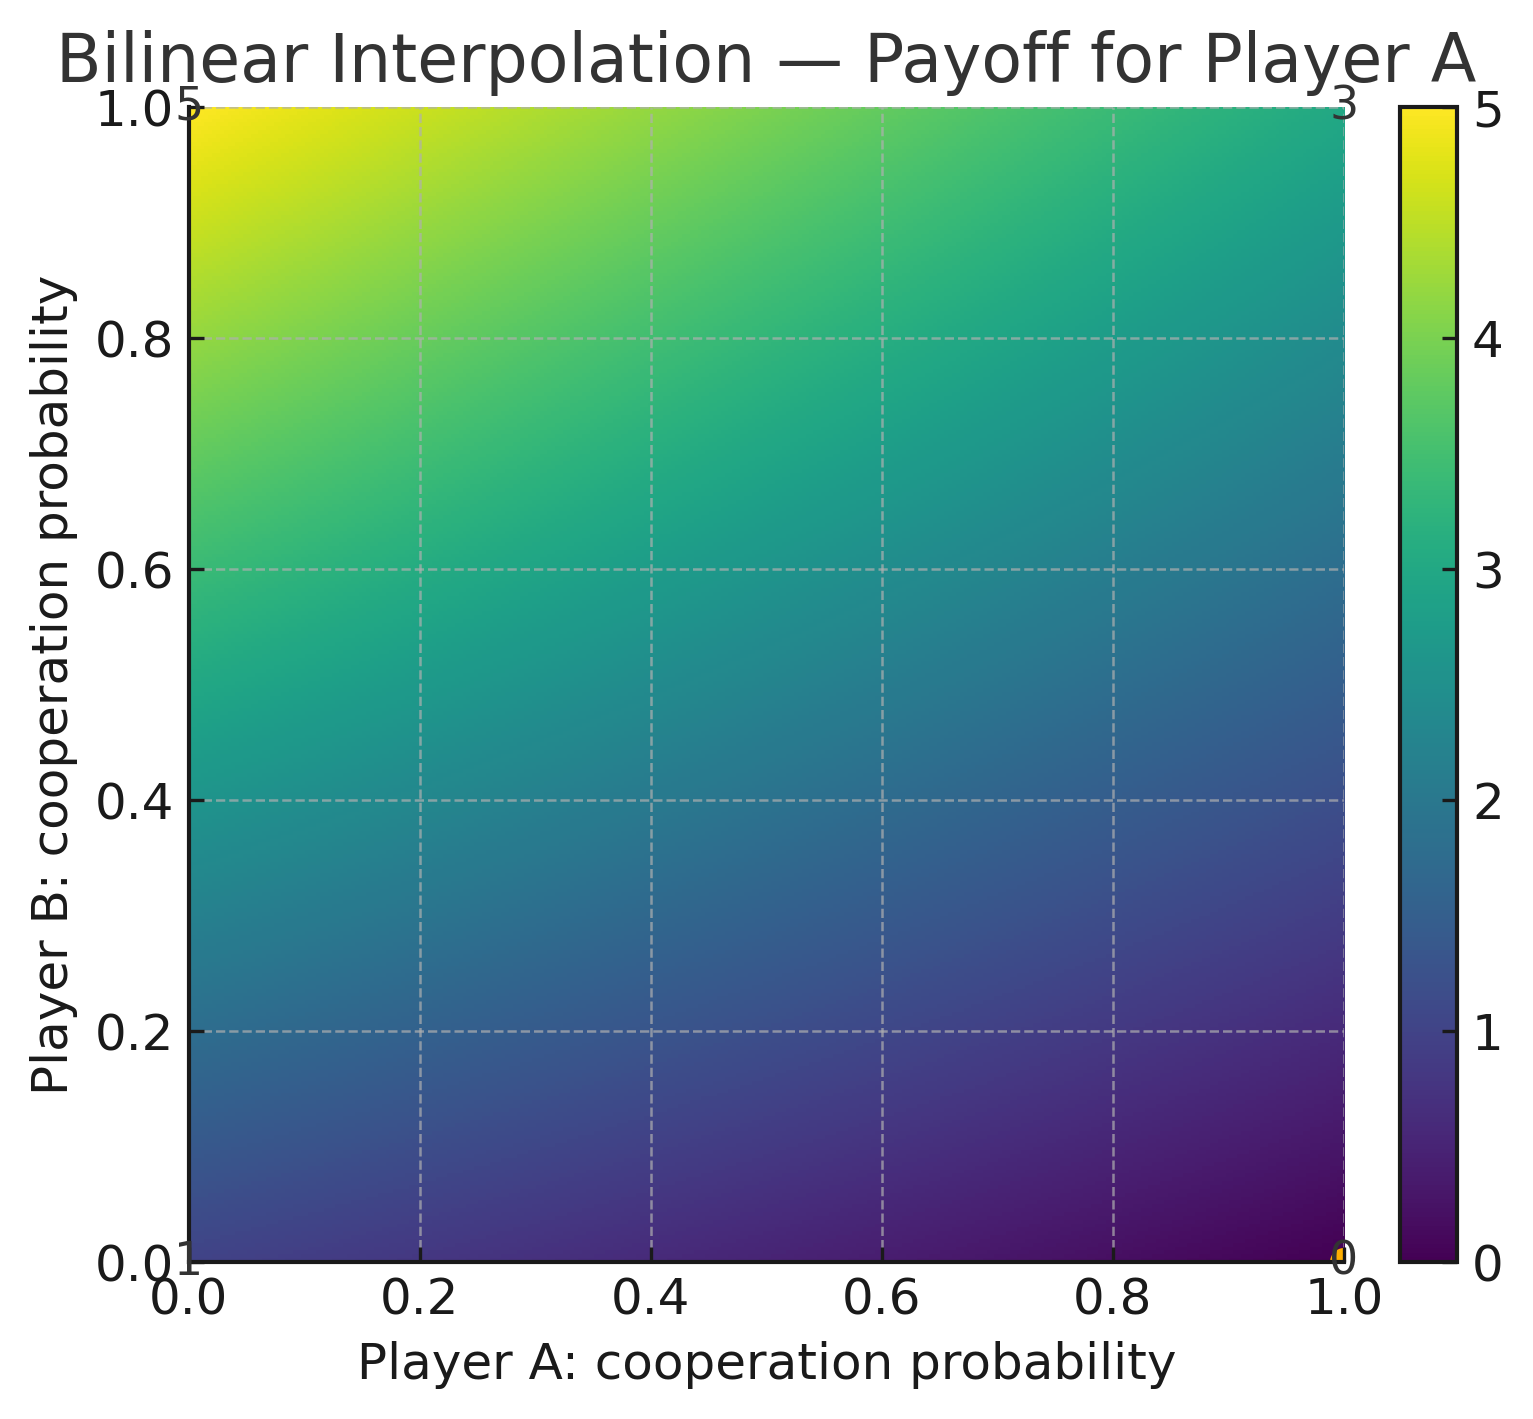
\includegraphics[width=0.45\textwidth]{images/pd_heatmap_A}\hfill
	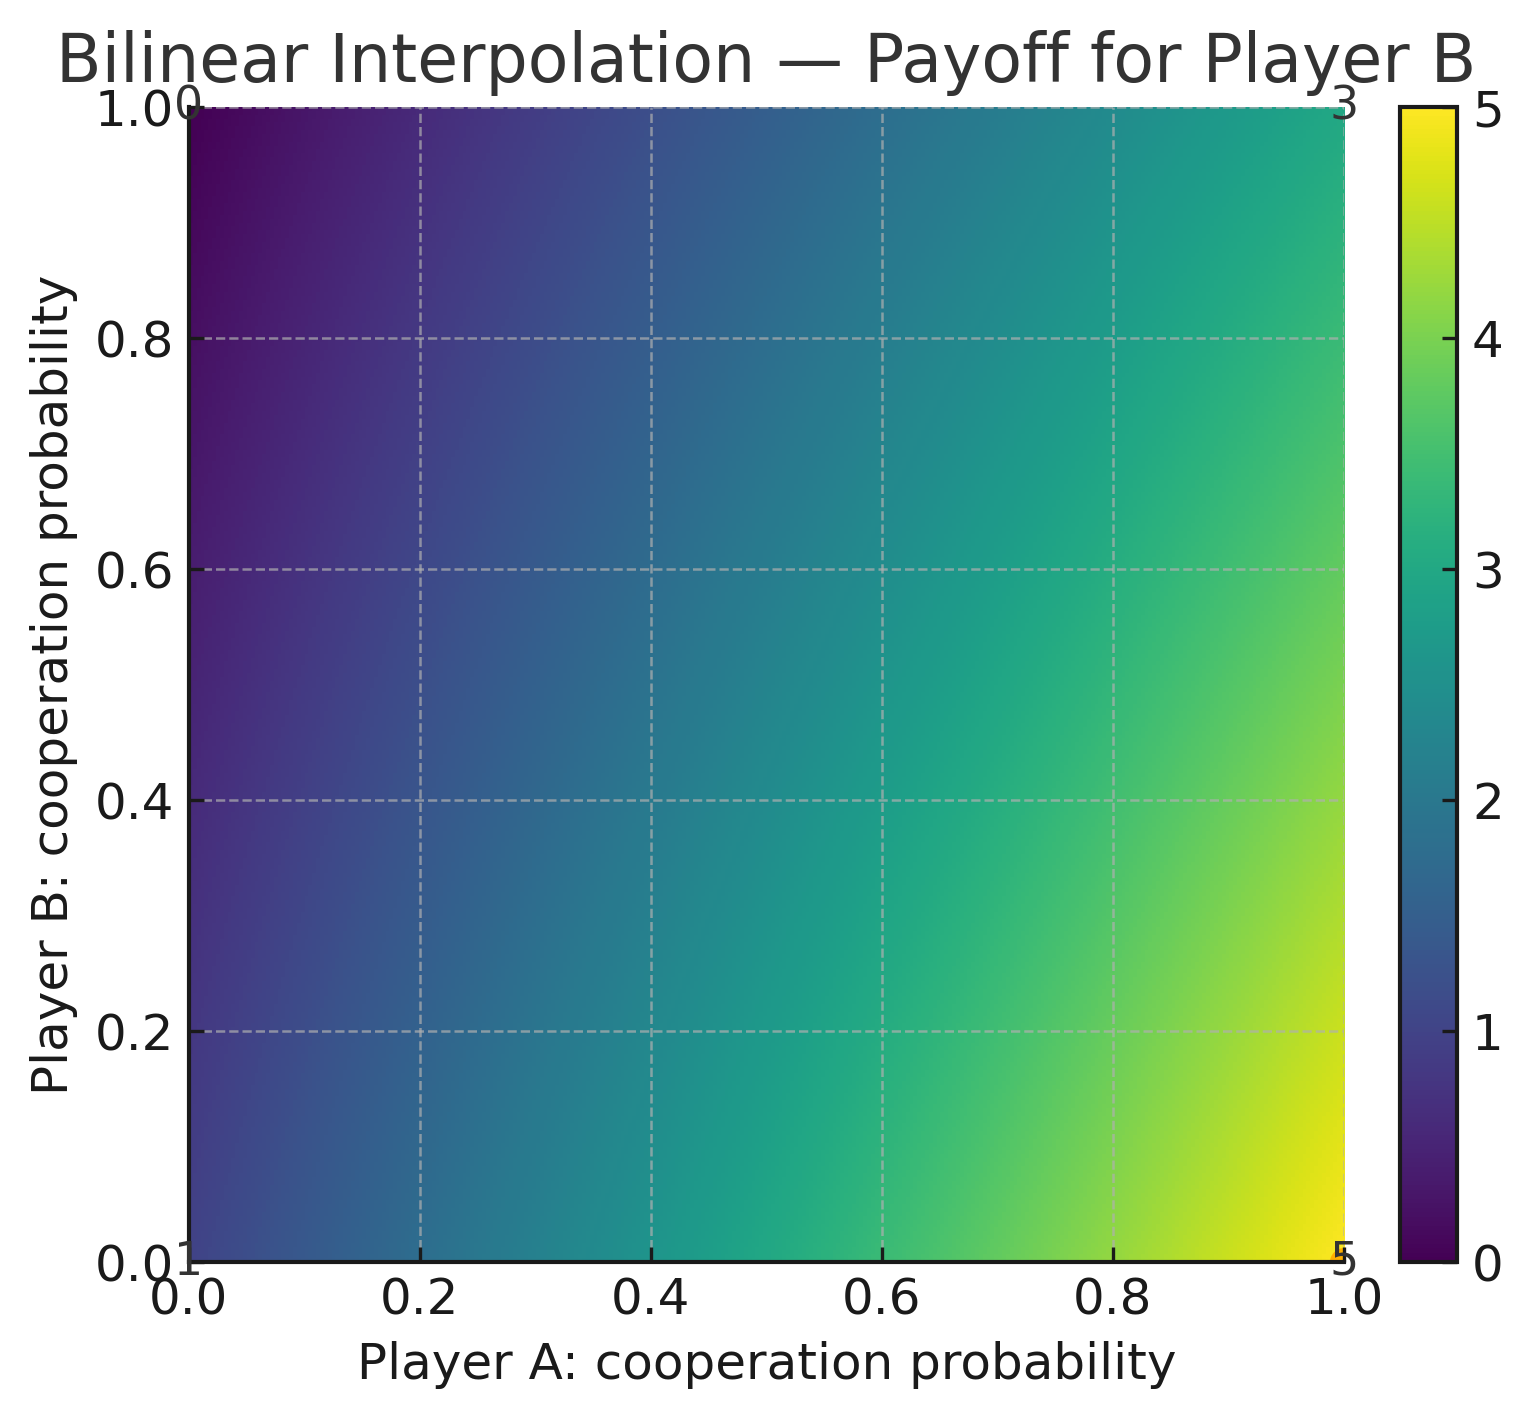
\includegraphics[width=0.45\textwidth]{images/pd_heatmap_B}
	\captionsetup{singlelinecheck=false}
	\caption{Pay-off heat maps in the ICPD.}
	\label{fig:heatmaps}
\end{figure}

% I used ChatGPT-o4 to generate these heat maps.
% It generated them using these functions:
%
% $$U_A = (1-x)(1-y)R_A + (1-x)yS_A + x(1-y)T_A + xyP_A$$
% $$U_B = (1-x)(1-y)R_B + (1-x)yS_B + x(1-y)T_B + xyP_B$$
%
% These functions are applied to every point on the map.
% The variable x is the investment of strategy A and y is the investment of strategy B.
The second approach utilises only equations instead.
This pay-off system of [sciencedirect.com] is formed by:

$$p_A = y - c \cdot x + c$$
$$p_B = x - c \cdot y + c$$

$p_A$ and $p_B$ are the pay-offs of strategy A and B respectively.
$x$ is the investment of strategy A and $y$ is that of strategy B.
The coefficient $c$ ranges, as well as x and y, from 0 to 1 and describes the cost-to-benefit ratio.
The pay-off is highly influenced by the opponent's investment.
Only a fraction of one owns contribution is subtracted, $c$ being the coefficient.
The minimum pay-off one strategy can collect is then $-c$.
To avoid negative pay-offs and enhance subsequent convenience, a third addend is appended, $c$.
So, the least points that can be gained is 0.
The maximal points, which can be earned by exploitation, is $1 + c$.


% Let's see if the principles of the initial PD are still valid.
% It is better for one to defect (submit a 0) to get rid of the subtraction.
% And it is better for the strategy if the opponent's cooperates.
% If both defect, one gets zero points.
% If both cooperate, both get one point.
% If, however, one strategy exploits the opponent, meaning it defects while the other cooperates, it will get the maximum points being 1.
% The opponent would then get $-c$ points.
% This is the least one can receive.

		% 0 to 1 rather than cooperation or defection\\
		% Pay-off system\\ % https://www.sciencedirect.com/science/article/pii/S0022519306004255?casa_token=hIA0lYvzjf8AAAAA:Up2uQ89wotaLz7s1R0dM2FK7SaulAo40wIM-BdM9yooZ8uJeRL6mPs-K55dPNGs4XkcclNVjDQ#aep-section-id24
		% more accurate\\
		% more complex, generates more data \textrightarrow more insightful\\

\subsection{Additional variants}

There exist several extensions of the PD that will remain untouched in this thesis, one of which is noise, meaning that investments are altered with a certain probability.
This noise is introduced to simulate misunderstandings.\\
Another advancement being the alternating form.
In this variant, investments are contributed in succession rather than concurrently as in the conventional simultaneous model.\\
The evolutionary research domain surveys the success of strategies in a world where natural selection takes place.
This implies that losing strategies vanish, while successful ones replicate.

% \subsection{Noise}
%
% Noise in the ICPD is the equivalent to miscommunication or misunderstanding in the real world.
% In this variant of the PD, noise is essential to trigger interesting outcomes.
% When a game of the ICPD is started and two strategies who start with a full investment, many strategies only respond with full investments.
% So noise is necessary to trigger continuous investments. 
% Without noise, in many cases, the ICPD would be equivalent to the IPD.
%
% 		% sometimes necessary to trigger continuous investments\\
% 		% simulates misunderstandings\\
%
% \subsection{Simultaneous vs Alternating}
%
% Two main differences can be seen when simulating an iterated variant of the PD.
% On one hand there is the simultaneous form whereby the strategies submit their contribution at the same time.
% On the other hand, there is the alternating form in which on e strategy submits its contribution and the other strategy can respond to this contribution is that round.
% Since the alternating form gives and advantage to the strategy which is allowed to respond, this only makes things more complicated than necessary.
% So, this analysis is only dedicated to the simultaneous form.

\subsection{Current Findings}

Axelrod's Tournament
In the simpler variants, e.g. the IPD without noise, it has been proved many times over that the strategy Tit-For-Tat is the most successful one. [sources]
The success of strategies, however, can vary depending on certain conditions such as the influence of noise or different pay-off systems where continuous investments can be submitted.
So, the very specific area of the simultaneous ICPD, has not been very well explored.
...

\section{Methods and Implementation}

For answering the central research question, it was necessary to develop a overarching study design (3.1), to specify the strategies that will be pursued in the iterated continuous Prisoner’s dilemma (3.2), and to determine details of the implementation in terms of IT (3.3).

\subsection{Study design}

Erratic behaviour in respect of the PD can be equated to a random conduct.
Three strategy-types are proposed by reason that counter such erraticism.
Hereunto can a strategy either be unaffected and behold its manner of responding or react to the randomness.
In the former case, strategies are identified as rigid.
Whereas the latter is characterised as adaptive.\\

All of these categories of behaviour can algorithmised differently.
This particularly concerns the above introduced distinction of the discrete and the continuous form.
Applied to the erratic strategies, this means that the investment is a substantial random number between zero and one.
In contrast, the discrete version of this strategy generates a random number that is then rounded to the nearest integer.
The same approach hold true in the adaptive strategy.
Discrete contributions of rigid strategies are equal to either always cooperating (AlwaysCooperate) or constantly defecting (AlwaysDefect).
Whereas continuous strategies of the rigid category contribute continuous investments invariably, e.g. 0.5 (AlwaysNeutral).\\

Furthermore, it is possible to specify the extremeness of each behaviour.
This means that the randomness of an erratic strategy, the adaptiveness of an adaptive strategy and the investment of a rigid strategy can be defined.
On this account, a parameter is incorporated into the determination of the investment and the evaluation of various conditions.
It has, incidently, never been undertaken in this manner in the history of researches that concern the ICPD.\\

To keep the number of comparisons manageable within the realms of a Maturaarbeit (MA), five strategy were chosen.
Firstly, the selected strategies in the random class were named to be a discrete (Random-Discrete) and a continuous (Random-Continuous) version.
Secondly, the same concept was established in the adaptive category with the discrete (Adapt-Discrete) and the continuous (Adapt-Continuous) behaviour.
These strategies hold a parameter which determines the peculiarity level and ranges from zero to ten.
So ultimately, the discrete and the continuous implementation are included in one strategy (AlwaysSame) due to this parameter.
Thus, the distinction of a discrete and a continuous design would be trivial.\\


% Surfaces:\\
%
% The end result of this paper will be several surface plots.
% The data will be generated by letting two parameter-based strategies play against each other the ICPD.
% The game will be structured so that every parameter came against every other parameter in the ICPD.
% In total, I will let them play the ICPD 100 times in order to smooth out abnormalities which happen only once.
% Like this, a surface can be plotted by having the x-axis being the parameter of strategy 1 and the y-axis being the parameter of strategy 2.
% The z-axis will indicate the points one strategy gained.
% Since there are two strategies in one game, one surface will be shown for each strategy.
% Further more, the two z-axis of the two surfaces can be added and form a new surface which shows the overall points gained by both strategies.
% The complement to that would be to subtract the two z-axis to plot a surface showing the difference between the two surfaces.
% This describes how much better one strategy was than the other.
% So, in the end there will be four surface plots per one ICPD.
%
		% Let two strategies play ICPD\\
		% let every parameter play against every other parameter\\
		% parameters as x and y-axis, points as z-axis\\
		% one surface for each strategy\\
		% overall surface is population wealth (addition)\\
		% difference surface is individual competence (subtraction)

\subsection{Implemented Strategies}

As justified before, five strategies, namely Random-Discrete, Random-Continuous, Adapt-Discrete, Adapt-Continuous and AlwaysSame, will be presented and specified in the following.
	
% 		\\My selection:\\
% In this simulation, strategies have to be defined and selected.
% There are two main points I want to investigate in this project.
% First, I want to associate the strategies to specific groups that differ in the characteristic of each member.
% I suggest the following three characteristics:
% \\1. Responsive
% \\2. Rigid
% \\3. Random\\
% I chose these three qualities due to the fact that one has to follow one of these three natures.
% In the real world, every personality can be associated with one of my defined groups.
% It can also be looked at this from another perspective.
% Whenever one has to respond to another's action, one has to decide how to answer.
% The shift applied to the previous investment can be categorised in one of these three groups.
% Either the shift is conditional to the opponent's last contribution, then this strategy is responsive.
% Or the shift is always 0 then the behaviour falls into the group of the rigid.
% This means that the investment will unconditionally stay the same.
% Or the shift is neither one of the above, meaning it doesn't depend on the past interactions nor stays it always 0.
% Then there cannot any determine aspect be established, meaning it is random.
% \\Second, the question arises if there is a difference between the ICPD and the IPD.
% So, I propose a discrete and a continuous variant of each group.
% With the exception of the group 'Rigid', there will be two members of each group.
% It will be clarified why only one strategy in this group makes sense.
% Thus, we can analyse the difference between the two members of the group to clarify which variant gained more points in the ICPD.
% Having two strategies in each group except in the group 'Rigid', means implementing five strategies.
% And letting all strategies play against every other strategy, including itself, means having enough data to plot $4 \cdot \sum_{a=1}^{5}$ surfaces.
% In total, this would equal to 60 surface plots.\\
% The following strategies are described by algorithmising them.
% $i(\theta)$ is a function that corresponds to the investment in the current round and holds the variable $\theta$ which is the parameter of the strategy in this round.
% I showcase what the behaviour of the strategy will be equivalent to when the parameter is 0, 5 and 10 for an easier understanding.\\
% 		\\Mean:\\
% The strategy Mean belongs to the group of the responsive strategies.
% It takes the investments of the opponent in the last $\theta_{\mathrm{Mean}}$ previous rounds as variables to its function to calculate the mean.
% This mean will then be submitted in the next round.
% Since in the first $\theta_{\mathrm{Mean}}$ rounds the strategy cannot calculate an average, it will submit full cooperation to offer maximum points for both of them.
% $$i(\theta_{\mathrm{Mean}}) = \frac{1}{\theta_{\mathrm{Mean}}}\sum_{k=1}^{\theta_{\mathrm{Mean}}}\bar i_k$$
% The variable $\bar i_k$ is the $k$'th element of the history of the opponent's investments, $k = 1$ being the last round.
% This strategy, Mean, with the parameter 0 is equivalent to  since it only calculates the mean of the last opponent's submission.\\
\begin{itemize}
	\item
Adapt-Continuous (AdpC) is an, as the name suggests, adaptive and thus responsive strategy.
It starts with full cooperation to offer a constructive relationship within this simulation.
After having played one round, it will adapt to the submissions of the opponent by shifting its own investment towards the opponent's.
$$i(\theta_{\mathrm{AdpC}}) = i_1 + s(\theta_{\mathrm{AdpC}})$$
$$s(\theta_{\mathrm{AdpC}}) = \frac{\theta_{\mathrm{AdpC}}}{5} \cdot (\bar i_1 - i_1)$$
The shift being applied to its own previous investment is notated with the function $s(\theta_{\mathrm{AdpC}})$.
This strategy with the parameter 0 is identical to AlwaysCooperate since the difference and thus the shift is multiplied by 0.
Dividing $\theta_{\mathrm{AdpC}}$ by 5 implies the fact that this coefficient to the difference is equal to one if the parameter equals five.
This means that the strategy will shift its next investment to exactly the previous investment of the opponent.
This behaviour corresponds to Tit-For-Tat.
$\theta_{\mathrm{AdpC}} = 10$ also shows an interesting nature of the strategy.
By having the parameter set to ten, it means Adapt will add the shift to its own previous investment twice.
Of course, one strategy is not allowed to submit any investment that exceeds the limits that is defined to be from 0 to 1.
The implementation of this strategy will simply set its investment to the reached limit if surpassed.\\

\item 
As I mentioned, there is one continuous and one discrete strategy.
This means there must be an Adapt-Discrete (AdpD) implemented.
The simplest implementation of this strategy is to take the same investment function as Adapt-Continuous and round the result.
$$i(\theta_{\mathrm{AdpD}}) = \round{i_1 + s(\theta_{\mathrm{AdpD}})}$$
$$s(\theta_{\mathrm{AdpD}}) = \frac{\theta_{\mathrm{AdpD}}}{5} \cdot (\bar i_1 - i_1)$$
Something that is not seen in these equations is that the strategy will start with full cooperation, as Adapt-Continuous.
If $i(\theta_{\mathrm{AdpD}}) \ge 0.5$, the ultimate investment will be 1.
Otherwise it will be equal to 0.
Once the strategy is at full defection, it can only get to cooperation again if $\theta_{\mathrm{AdpD}} \ge 3$.
Here is why:\\
The maximum difference there can be is when this strategy submits 1 and the opponent submits a 0, so 1.
Looking at the function, this threshold of 0.5 can only be overstepped if the shift is at least equal to 0.5.
This only can be achieved if the coefficient is greater of equal to 0.5 ($\frac{\theta_{\mathrm{AdpD}}}{5} \ge 0.5$).
This inequation is fulfilled if $\theta_{\mathrm{AdpD}} \ge 3$.\\
$\theta_{\mathrm{AdpD}} = 0$ means, as in the continuous version, that the strategy corresponds to AlwaysCooperate because the shift is equal to 0 and thus always stays at its first investment, being full cooperation.
If the parameter is equal to 10, it is most likely to jump from 1 to 0 back to 1 and so on.
This only doesn't happen if the difference is less or equal to 0.25.\\

\item
AlwaysSame's (AlwS) parameter calculates the investment very simply.
The investment follows the equation: 
$$i(\theta_{\mathrm{AlwS}}) = \frac{\theta_{\mathrm{AlwS}}}{10}$$
This means that after each incrementation of the parameter, the investment increases by 0.1.
Parameter 0 is equivalent to AlwaysDefect and parameter 1 has the same behaviour as AlwaysCooperate.
If the parameter is set to five, the strategy will always submit the investment 0.5 which is identical to Neutral.\\

\item
The other strategy in the group of the random is oppositely continuous, meaning it can additionally submit any number between 0 and 1.
The name of this strategy is logically Random-Continuous (RndC).
This strategy has a base being at 0.5.
The parameter defines the shift being applied to the base, calculated by the equation:
$$i(\theta_{\mathrm{RndC}}) = 0.5 + \epsilon \cdot s(\theta_{\mathrm{RndC}})$$
$$s(\theta_{\mathrm{RndC}}) = \frac{\theta_{\mathrm{RndC}}}{20}$$
$$\Pr(\epsilon = 1) = \Pr(\epsilon = -1) = \frac{1}{2}$$
$s$ means the shift.
It is divided by 20 so the maximum shift, parameter being 10, can not exceed the range of 0 and 1.
There is a 50\% probability of subtracting or adding this shift, indicated by the symbol $\epsilon$.\\

\item
Random-Discrete (RndD) is a strategy in the group of the random.
It is also discrete, meaning it can only submit either 0 or 1.
The parameter in this strategy determines the likelihood of submitting 0 and 1 respectively.
The probability of submitting full defection is described in the following equation.
$$
\begin{array}{c}
i(\theta_{\mathrm{RndD}}) = \Pr(i = 1 \mid \theta_{\mathrm{RndD}}) = \frac{\theta_{\mathrm{RndD}}}{10}\\
\mathrm{or}\\
i(\theta_{\mathrm{RndD}}) = \Pr(i = 0 \mid \theta_{\mathrm{RndD}}) = 1 - \frac{\theta_{\mathrm{RndD}}}{10}
\end{array}
$$
Parameter 0 is equivalent to AlwaysDefect since the probability of submitting 0 is 0\%.
And on the other hand, parameter 10 is equivalent to AlwaysCooperate since the probability of submitting 1 is 100\%.\\
\end{itemize}

\begin{center}
\begin{tabular}{ c|c|c|c }
   & $\theta = 0$ & $\theta = 5$ & $\theta = 10$ \\ 
   \hline
	Random-Discrete & AlwaysDefect & - & AlwaysCooperate \\  
   \hline
	Random-Continuous & AlwaysNeutral & - & Random-Discrete ($\theta = 5$) \\
   \hline
	Always-Same & AlwaysDefect & AlwaysNeutral & AlwaysCooperate \\
   \hline
	Adapt-Discrete & AlwaysCooperate & - & -\\
   \hline
	Adapt-Continuous & AlwaysCooperate & Tit-For-Tat & -
\end{tabular}
\end{center}

\subsection{Implementation Details}

Regarding the initial problem of this thesis, both Random-Discrete and Random-Continuous play against every strategy (including themselves).
As there are eleven parameter values for each strategy, there will be $2 \cdot 5 \cdot 11 \cdot 11 = 1210$ encounters and thus comparisons.
20 iterations of the ICPD has been decided to suffice.
In addition, this game of 20 iterations is played a 100 times to flatten non-recurring abnormalities.
To avoid gratuitous huge numbers, the mean of the ultimate points of these 100 repetitions is taken.
This comes down to $100 \cdot 20 \cdot 1210 = 2420000$ procedures of the continuous PD.\\

One encounter of the $11 \cdot 11$ parameter-based ICPD (pbICPD) is displays in form of a surface.
There are two surfaces for each pbICPD, both of which represent the gained points of the corresponding strategy.
Additive, two farther surfaces can be established.
These ones are calculated by subtracting the gained-points surfaces and depict the relative gained, i.g. how much better was strategy A against strategy B.
Ultimately, a fifth surface will be generated by adding the two gained-points surfaces.
They illustrate the overall gain, meaning the points that have been gained in the game.


The simulation, data generation and visualisation is completely written in Python (version 3.13.5).
For the visualisation, as in generating the surface plots, a python library was used, namely Plotly.
More information about the python scripts and data visualisation files that were used can be found in the Appendix.
% If anyone is interested in simulating the project on their machine, they can go on my GitHub page and follow the instructions there:
% \href{https://github.com/adho08/Prisoner-s-Dilemma}{https://github.com/adho08/Prisoner-s-Dilemma}

	% \item Implemented Variants:\\
	% 	Prisoner's Dilemma\\
	% 	Iterated Prisoner's Dilemma\\
	% 	Iterated Continuous Prisoner's Dilemma\\
	% 	Parameter-Based Strategies\\
	% 	only PBS important for MA\\
	


\section{Results}

\begin{wrapfigure}{l}{0.25\textwidth}
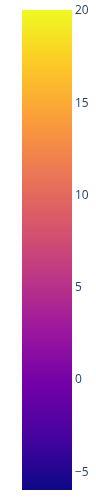
\includegraphics[height=3cm]{plots/Colorscales/Plasma.png}{Plasma}
\caption{Colour scale for the 'Gained Points' surfaces}
\label{fig:Plasma}
\end{wrapfigure}
In the following two pages, you will see all the surfaces of both Random-Discrete and Random-Continuous.
There are five surfaces in each interaction that are generated from one ICPD.
The x-axis, the one in be bottom-right, shows the parameter of the main strategy.
The y-axis, the other axis on the bottom, indicates the parameter of the opponent.
The z-axis always shows the points.
All the surfaces are not only marked by height but also by colour.
The context in which points are displayed depends on the surface. 
The first two rows are the most basic surface plots.
They show the gains of the strategy itself and the opponent's.
The highest point that can appear is at 30.
And the lowest is at 0.
The maximum can be calculated by regarding the pay-off equations.
The maximum points are gained by exploitation.
So, $P_A =  y - c \cdot x + c$ becomes by substitution $P_A = 1 - 0.5 \cdot 0 + 0.5$ \textrightarrow $P_A = 1.5$.
And since the CPD is played 20 times, $P_A \cdot 20 = 30$.
So, the boundaries in which the points can vary is from 0 to 30.
All the points, that are at height 20, have their correspondence in the other surface since in order to get 20 points, mutual cooperation is required.
The same principle can be allied to the maximum, minimum points and mutual defection which is at height 10.
Wherever a minimum point can be seen, the correspondence is the maximum point at the same x-y-coordinate.
The colour of the points indicates the same as the height, the number of points.
So, one can read this surface more accurately by regarding Figure \ref{fig:Plasma}.
The next two surfaces concern the advantage one strategy has over the other.
This shows us how much more one strategy had over the other.
For the surface of the main strategy, simply the opponent's surface is subtracted from it's surface and vice versa.
The maximum and the minimum can be calculated by taking the difference of the maximum and the minimum of the first two surfaces.
So, the points can vary between -30 and 30.
(30 - 0 = 30, 0 - 30 = -30)
The two initial surfaces would intersect if they were put into one coordinate system.
The intersection is at all the locations where the both strategies have gained an equal amount of points.
At this location of the intersection, the surface plot, that demonstrates the advantage, would intersect with the zero-plane because the difference of two same number is always equal to zero.\\
The two advantage surfaces are always mirrored by the zero-plane since every time you subtract $A-B$, it is the same as $(B-A) \cdot -1$.\\
If this surface plot happens to be completely over the zero-plane, it means that the displays strategy has won every game they have played.
Also here, there is a colour scale.
This colour scale, however, differs from the first one.
I chose to use different colour scales for visualisation purposes due to the fact that the advantage surfaces have a different z-axis range than the first two.
(-30 to 30)
B)
% 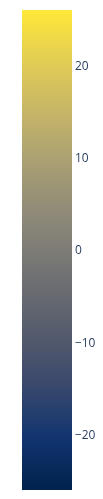
\includegraphics[height=3.0cm]{plots/Colorscales/Cividis.png}
The last row of surfaces displays how much points have been gained by both.
To generate these surfaces, one must add the surfaces which describe how much one has gained of the concerned strategies.
Looking at the pay-off equations, a point can not be over the limit of 20.
Both gain the most if both cooperate.
Following the equations, one gets 1 point after every round.
Since 20 rounds are played in total, the maximum is at 20.
(20 rounds * 1 point = 20 points)
I decided to also plot this surface to demonstrate the population welfare.
This means that the higher the points, the most have gained both together.
This plot has, as the advantage surfaces, a different z-axis range.
So a new colour scale is introduced.
C)
\newpage

% 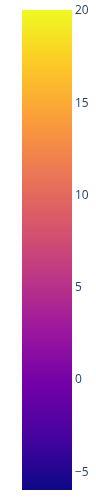
\includegraphics[height=3cm]{plots/Colorscales/Plasma.png}
% 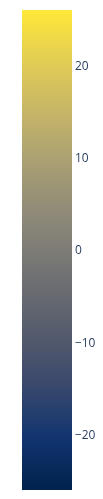
\includegraphics[height=3cm]{plots/Colorscales/Cividis.png}
% 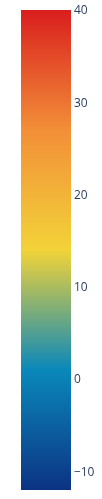
\includegraphics[height=3cm]{plots/Colorscales/Portland.png}

\newpage

\def \w {0.16}
\def \a {45}

% ------------------------------- Random-Discrete -------------------------------
Random-Discrete\\
\begin{figure}[h]
    \centering
    
    % Header row
    \begin{tabular}{p{0.7cm}ccccc}
        & \rotatebox{45}{Random-Discrete} & \rotatebox{45}{Random-Continuous} & \rotatebox{45}{AlwaysSame} & \rotatebox{45}{Adapt-Discrete} & \rotatebox{45}{Adapt-Continuous} \\[1cm]
        
        % Gain Random-Discrete row
        \rotatebox{90}{\parbox{2cm}{\centering Gain \\ Random-Discrete}} &
        \includegraphics[width=\w\textwidth]{plots/Random-Discrete/Random-Discrete_vs_Random-Discrete_2/Random-Discrete.png} &
        \includegraphics[width=\w\textwidth]{plots/Random-Discrete/Random-Discrete_vs_Random-Continuous/Random-Discrete.png} &
        \includegraphics[width=\w\textwidth]{plots/Random-Discrete/Random-Discrete_vs_AlwaysSame/Random-Discrete.png} &
        \includegraphics[width=\w\textwidth]{plots/Random-Discrete/Random-Discrete_vs_Adapt-Discrete/Random-Discrete.png} &
        \includegraphics[width=\w\textwidth]{plots/Random-Discrete/Random-Discrete_vs_Adapt-Continuous/Random-Discrete.png} \\[0.5cm]
        
        % Gain Opponent row  
        \rotatebox{90}{\parbox{2cm}{\centering Gain \\ Opponent}} &
        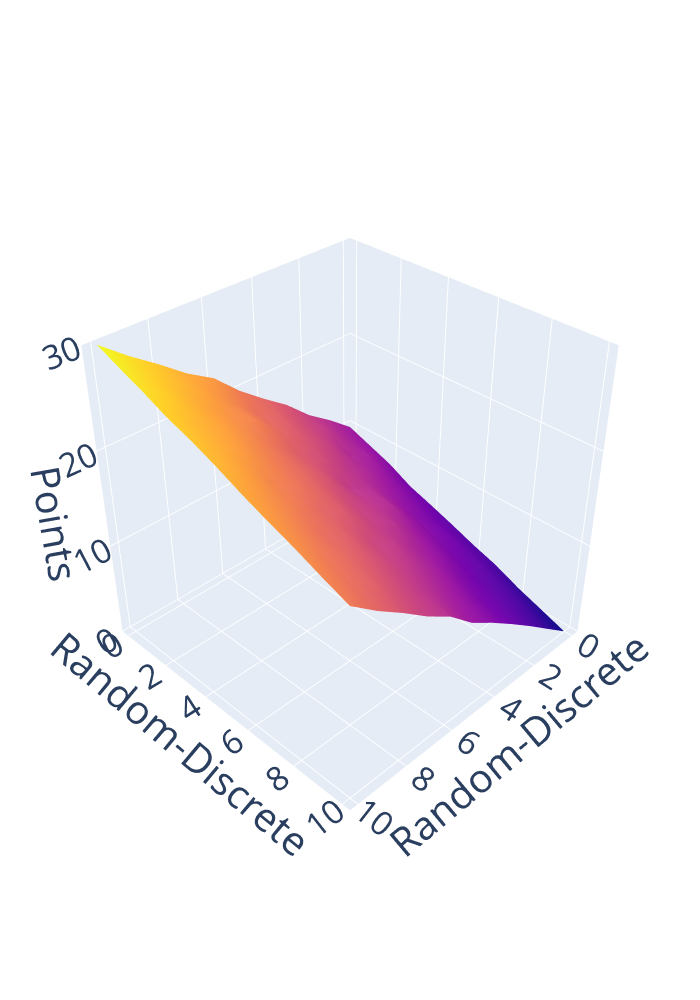
\includegraphics[width=\w\textwidth]{plots/Random-Discrete/Random-Discrete_vs_Random-Discrete_2/Random-Discrete_2.png} &
        \includegraphics[width=\w\textwidth]{plots/Random-Discrete/Random-Discrete_vs_Random-Continuous/Random-Continuous.png} &
        \includegraphics[width=\w\textwidth]{plots/Random-Discrete/Random-Discrete_vs_AlwaysSame/AlwaysSame.png} &
        \includegraphics[width=\w\textwidth]{plots/Random-Discrete/Random-Discrete_vs_Adapt-Discrete/Adapt-Discrete.png} &
        \includegraphics[width=\w\textwidth]{plots/Random-Discrete/Random-Discrete_vs_Adapt-Continuous/Adapt-Continuous.png} \\[0.5cm]
        
        % Advantage Random-Discrete row
        \rotatebox{90}{\parbox{2cm}{\centering Advantage \\ Random-Discrete}} &
        \includegraphics[width=\w\textwidth]{plots/Random-Discrete/Random-Discrete_vs_Random-Discrete_2/Random-Discrete_diff.png} &
        \includegraphics[width=\w\textwidth]{plots/Random-Discrete/Random-Discrete_vs_Random-Continuous/Random-Discrete_diff.png} &
        \includegraphics[width=\w\textwidth]{plots/Random-Discrete/Random-Discrete_vs_AlwaysSame/Random-Discrete_diff.png} &
        \includegraphics[width=\w\textwidth]{plots/Random-Discrete/Random-Discrete_vs_Adapt-Discrete/Random-Discrete_diff.png} &
        \includegraphics[width=\w\textwidth]{plots/Random-Discrete/Random-Discrete_vs_Adapt-Continuous/Random-Discrete_diff.png} \\[0.5cm]
        
        % Advantage Opponent row
        \rotatebox{90}{\parbox{2cm}{\centering Advantage \\ Opponent}} &
        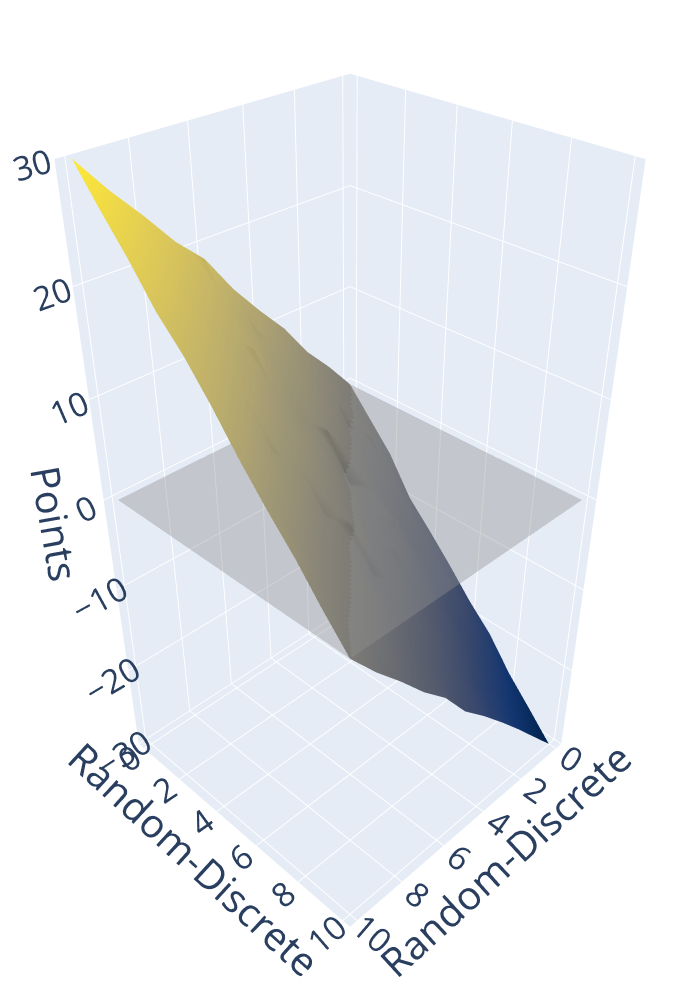
\includegraphics[width=\w\textwidth]{plots/Random-Discrete/Random-Discrete_vs_Random-Discrete_2/Random-Discrete_2_diff.png} &
        \includegraphics[width=\w\textwidth]{plots/Random-Discrete/Random-Discrete_vs_Random-Continuous/Random-Continuous_diff.png} &
        \includegraphics[width=\w\textwidth]{plots/Random-Discrete/Random-Discrete_vs_AlwaysSame/AlwaysSame_diff.png} &
        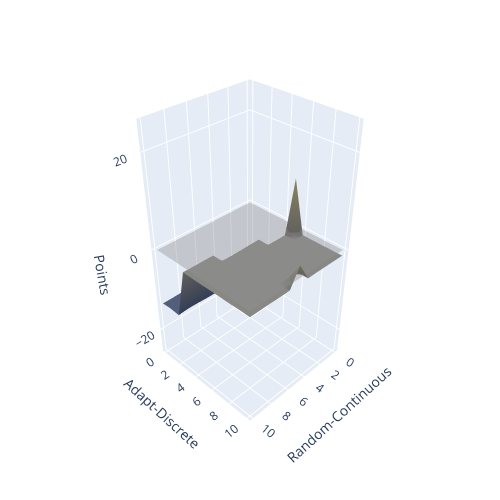
\includegraphics[width=\w\textwidth]{plots/Random-Discrete/Random-Discrete_vs_Adapt-Discrete/Adapt-Discrete_diff.png} &
        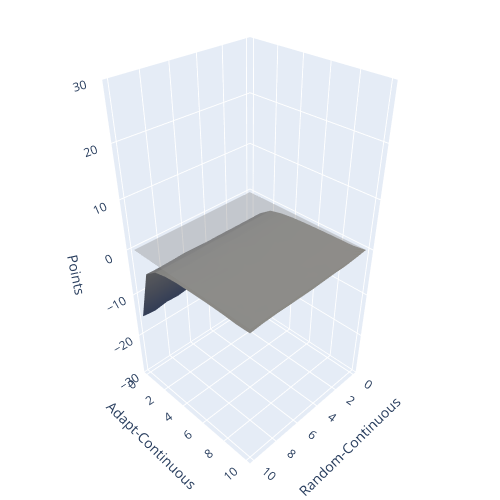
\includegraphics[width=\w\textwidth]{plots/Random-Discrete/Random-Discrete_vs_Adapt-Continuous/Adapt-Continuous_diff.png} \\[0.5cm]
        
        % Overall Gain row
        \rotatebox{90}{\parbox{2cm}{\centering Overall \\ Gain}} &
        \includegraphics[width=\w\textwidth]{plots/Random-Discrete/Random-Discrete_vs_Random-Discrete_2/added.png} &
        \includegraphics[width=\w\textwidth]{plots/Random-Discrete/Random-Discrete_vs_Random-Continuous/added.png} &
        \includegraphics[width=\w\textwidth]{plots/Random-Discrete/Random-Discrete_vs_AlwaysSame/added.png} &
        \includegraphics[width=\w\textwidth]{plots/Random-Discrete/Random-Discrete_vs_Adapt-Discrete/added.png} &
        \includegraphics[width=\w\textwidth]{plots/Random-Discrete/Random-Discrete_vs_Adapt-Continuous/added.png} \\
    \end{tabular}
    
\end{figure}

\newpage
% ------------------------------- Random-Continuous -------------------------------
\begin{figure}[h]
    \centering
    
    % Header row
    \begin{tabular}{p{0.7cm}ccccc}
        & \rotatebox{45}{Random-Discrete} & \rotatebox{45}{Random-Continuous} & \rotatebox{45}{AlwaysSame} & \rotatebox{45}{Adapt-Discrete} & \rotatebox{45}{Adapt-Continuous} \\[1cm]
        
        % Gain Random-Continuous row
        \rotatebox{90}{\parbox{2cm}{\centering Gain \\ Random-Continuous}} &
        \includegraphics[width=\w\textwidth]{plots/Random-Continuous/Random-Continuous_vs_Random-Discrete/Random-Discrete.png} &
        \includegraphics[width=\w\textwidth]{plots/Random-Continuous/Random-Continuous_vs_Random-Continuous_2/Random-Continuous.png} &
        \includegraphics[width=\w\textwidth]{plots/Random-Continuous/Random-Continuous_vs_AlwaysSame/Random-Continuous.png} &
        \includegraphics[width=\w\textwidth]{plots/Random-Continuous/Random-Continuous_vs_Adapt-Discrete/Random-Continuous.png} &
        \includegraphics[width=\w\textwidth]{plots/Random-Continuous/Random-Continuous_vs_Adapt-Continuous/Random-Continuous.png} \\[0.5cm]
        
        % Gain Opponent row  
        \rotatebox{90}{\parbox{2cm}{\centering Gain \\ Opponent}} &
        \includegraphics[width=\w\textwidth]{plots/Random-Continuous/Random-Continuous_vs_Random-Discrete/Random-Continuous.png} &
        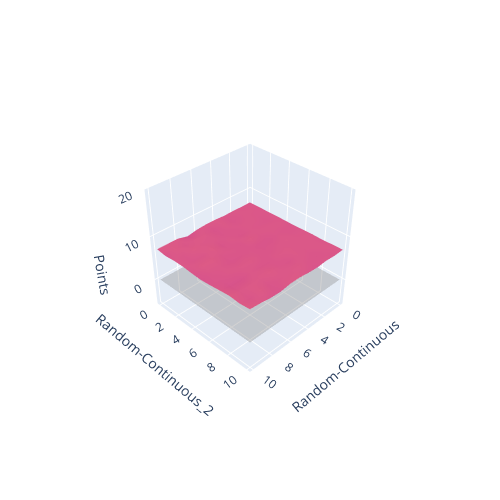
\includegraphics[width=\w\textwidth]{plots/Random-Continuous/Random-Continuous_vs_Random-Continuous_2/Random-Continuous_2.png} &
        \includegraphics[width=\w\textwidth]{plots/Random-Continuous/Random-Continuous_vs_AlwaysSame/AlwaysSame.png} &
        \includegraphics[width=\w\textwidth]{plots/Random-Continuous/Random-Continuous_vs_Adapt-Discrete/Adapt-Discrete.png} &
        \includegraphics[width=\w\textwidth]{plots/Random-Continuous/Random-Continuous_vs_Adapt-Continuous/Adapt-Continuous.png} \\[0.5cm]
        
        % Advantage Random-Continuous row
        \rotatebox{90}{\parbox{2cm}{\centering Advantage \\ Random-Continuous}} &
        \includegraphics[width=\w\textwidth]{plots/Random-Continuous/Random-Continuous_vs_Random-Discrete/Random-Continuous_diff.png} &
        \includegraphics[width=\w\textwidth]{plots/Random-Continuous/Random-Continuous_vs_Random-Continuous_2/Random-Continuous_diff.png} &
        \includegraphics[width=\w\textwidth]{plots/Random-Continuous/Random-Continuous_vs_AlwaysSame/Random-Continuous_diff.png} &
        \includegraphics[width=\w\textwidth]{plots/Random-Continuous/Random-Continuous_vs_Adapt-Discrete/Random-Continuous_diff.png} &
        \includegraphics[width=\w\textwidth]{plots/Random-Continuous/Random-Continuous_vs_Adapt-Continuous/Random-Continuous_diff.png} \\[0.5cm]
        
        % Advantage Opponent row
        \rotatebox{90}{\parbox{2cm}{\centering Advantage \\ Opponent}} &
        \includegraphics[width=\w\textwidth]{plots/Random-Continuous/Random-Continuous_vs_Random-Discrete/Random-Discrete_diff.png} &
        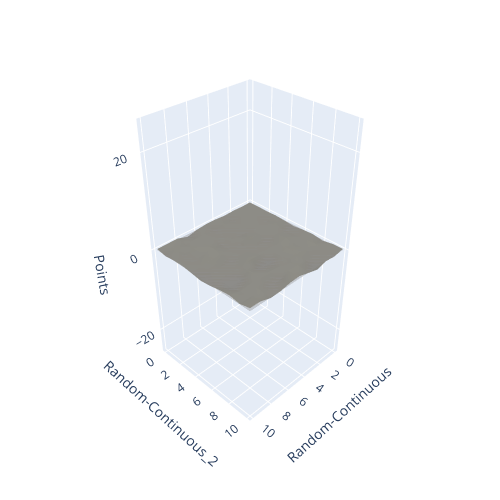
\includegraphics[width=\w\textwidth]{plots/Random-Continuous/Random-Continuous_vs_Random-Continuous_2/Random-Continuous_2_diff.png} &
        \includegraphics[width=\w\textwidth]{plots/Random-Continuous/Random-Continuous_vs_AlwaysSame/AlwaysSame_diff.png} &
        \includegraphics[width=\w\textwidth]{plots/Random-Continuous/Random-Continuous_vs_Adapt-Discrete/Adapt-Discrete_diff.png} &
        \includegraphics[width=\w\textwidth]{plots/Random-Continuous/Random-Continuous_vs_Adapt-Continuous/Adapt-Continuous_diff.png} \\[0.5cm]
        
        % Overall Gain row
        \rotatebox{90}{\parbox{2cm}{\centering Overall \\ Gain}} &
        \includegraphics[width=\w\textwidth]{plots/Random-Continuous/Random-Continuous_vs_Random-Discrete/added.png} &
        \includegraphics[width=\w\textwidth]{plots/Random-Continuous/Random-Continuous_vs_Random-Continuous_2/added.png} &
        \includegraphics[width=\w\textwidth]{plots/Random-Continuous/Random-Continuous_vs_AlwaysSame/added.png} &
        \includegraphics[width=\w\textwidth]{plots/Random-Continuous/Random-Continuous_vs_Adapt-Discrete/added.png} &
        \includegraphics[width=\w\textwidth]{plots/Random-Continuous/Random-Continuous_vs_Adapt-Continuous/added.png} \\
    \end{tabular}
\end{figure}

\newpage

\begin{itemize}

	\item Random-Discrete\textunderscore2:\\

		Gained points:\\
			First, it has to be mentioned that Random-Discrete behaves like AlwaysSame.
			This is due to the fact that I have run this simulation 100 times to smooth out one-time abnormalities.
			This is notable by looking at the column where Random-Discrete plays against AlwaysSame.
			These two columns look arguably alike.\\
			Since the two strategies behave exactly in the same way, these two surface plots are simply mirror-inverted by 45° on the x- and y-axis.
			The left and right corner are the extremes.
			Random-Discrete gets exploited when it has its parameter at 10, meaning it corresponds to AlwaysCooperate, and Random-Discrete\textunderscore2 has its at 0, i.e. it is equivalent to AlwaysDefect.
			This is how one can get the maximum output, by exploiting.
			This can be seen in the surface of Random-Discrete\textunderscore2.
			The behind corner is at the coordinate 0, 0.
			There, both defect constantly.
			This is the point where both get their relative lowest output, as can be seen later.\\
			The nearest point is at the coordinate 10, 10.
			The parameter 10 indicates the same behaviour as AlwaysCooperate.
			So, both always cooperate and thus have not a so high output as when they exploit but fairly enough.\\
		\\Advantages:\\
			This time, the surface is mirrored at the cutting edge at $z=0$.
			This is because both gain surfaces are mirrored.
			The absolute peaks of both derive from having the maximum output.
			Since one can get the maximum output only if the other gets exploited, the advantage surface result in the highest peak possible.
			When the two parameter's are identical, however, they are not any better than the other.
			This makes sense since they behave the same when they have the same parameter and can thus not exploit each other.\\
		\\Overall:\\
			Here, it is clearly visible that the hight point on the surface is when both cooperate.
			This illustrates the dilemma pretty well.
			It is better for both if they both cooperate, all the time.
			As already mentioned, the most behind point, being the lowest, results from the fact that both defected constantly.
			So, for the welfare of the population, it is best if both cooperate every round.

	\item Random-Continuous\\

		Gained points:\\
			This surfaces ranges from 20 to 10 continuously.
			It seems as the surface is not influenced by the parameter of Random-Continuous.
			This is logical and will be looked at the discussion.\\
			The second surface ranges from about 5 to 25.
			Also here the surface is only influenced by the parameter of Random-Discrete.
		\\Advantages:\\
			Both surfaces, when put together in one plot, would intersect exactly in the middle.
			Since they range from different limits but both upper and lower limit add up to 30, they intersect in the middle where the parameter of Random-Discrete is 5.
			That is why the surface of advantage intersects the zero-plane at the same line.
		\\Overall:\\
			Naturally, this surface is only influenced by the parameter of Random-Discrete and not Random-Continuous.
			It ranges continuously from 25 to 35.

	\item AlwaysSame\\
		This column of surfaces looks identical to the one against Random-Discrete\textunderscore2.
		In the discussion further investigation will be made.
		Since I have explained the properties of these surfaces already, I will not explain them again.

	\item Adapt-Discrete\\

		Gained points:\\
			In the surface of Random-Discrete against Adapt-Discrete, there is a stripe at the parameter of Adapt-Discrete being 0 to 2.
			The stripe ranges from absolute exploitation at (0, 0) to mutual cooperation at parameter of Random-Discrete being 10.
			Abruptly, this stripe does not follow its pattern in the x-direction any more.
			Rather a new slope is visible.
			This slope has its lowest points at 10.
			But, both slopes range from where they begin at the y-z-plane to 20 at the other y-z-plane.
			Remember that 20 is the result of mutual cooperation.
			As a result of that, there are also 20 points in the corresponding surface plot at the same x-y-coordinates.
			This is indeed the case.
			Also the maximum points of the first plot indicate that the same points on the other surface must be at height 0.
			The broader slope is also going downwards.
			But this slope is not as steep as the one on the other surface and thus has lower points at the edge where the parameter of Random-Discrete is 0.
			When Random-Discrete has its parameter at 10, which means it behaves like AlwaysCooperate, mutual cooperation will take place.\\

		Advantages:\\
			Since the slopes look pretty similar, there are practically no advantages in this area.
			At the coordinates of the stripe, however, is a great advantage which only Random-Continuous has over Adapt-Discrete.
			The advantage surface of Adapt-Discrete is not visible to see relevant part.
			The plane covers the inverted stripe of the advantage surface of Random-Discrete.
			The rest of the surface is very near to the zero-plane which means it was as good as Random-Continuous in this area.
		Overall:\\
			Of course, the maximum points are at the locations where mutual cooperation is held place (40).
			This stripe is, this time, not at steep as as the broader slope.
			The slope ends at the y-z-plane at height 20.\\

	\item Adapt-Continuous\\

		Gained points:\\
			Intuitively, the discrete stripe becomes a continuous curve.
			The edge where points are at height 20, stays as it was in the game against Adapt-Discrete.
			The broad slope is also similar to that surface, its lowest points being at 10.
			The surface of Adapt-Continuous is in a same way similar to the one of Adapt-Discrete.
			The edges are curved out.
			But, the slope is, again, a bit steeper than the one of Random-Discrete.\\
		Advantages:\\
			The same applies at the advantage surfaces.
			They simply are curvy instead of edgy.
			The advantage surface of Adapt-Continuous is in a difficult angle to see.
			The origin of the coordinate-system is the lowest point of this surface.
			I concluded this fact by knowing that the highest point of the other advantage surface has its correspondence at height 0.\\
		Overall:\\
			The maximum points are aligned in a line.
			More specific, an edge of the surface at height 40.
			The least points are gained at the edge more behind at the y-z-plane.
			This edge is rather a curve than a straight line.
			This curve bows from exploitation at coordinates being at (0, 0) to 20, the absolute minimum of this surface.
	
	\item Random-Discrete:\\

		This surface has already been explained.
		These are the same surfaces as when Random-Discrete played against Random-Continuous in the first figure.
	
	\item Random-Continuous\textunderscore2:\\

		Gained points:\\
			As already mentioned, Random-Continuous behaves like Neutral by having played several times.
			So, Random-Continuous will submit 0.5 always.
			This results to having a completely flat surface.
			We can calculate at which height the surface is.
			Plugging in 0.5 for both x and y in the pay-off equations, we get $P_A = 0.5 - c \cdot 0.5 + c$ where $c$ is, as always, equal to 0.5.
			The pay-off of strategy A is $P_A = 0.75$ and having played the ICPD 20 rounds, it is equal to $P_A \cdot 20 = 15$.
			Both strategies A and B get the same pay-off since they submitted the same investment.
			$P_B = P_A \rightarrow P_B \cdot 20 = 15$.
			So, both surfaces are at the same height at every point.

		Advantages:\\
			Subtracting two flat surfaces at the same height at every coordinate, gives you a also flat surface which corresponds to the zero-plane.
			No strategy was better than the other at any point.

		Overall:\\
			Adding these even two surfaces which are both at height 15, gives you a surface at height $15 + 15 = 30$.

	\item AlwaysSame:\\

		These surfaces are identical to the one's of the Random-Continuous vs. Random-Discrete interaction.
		I will not describe them as they already have been.
	
	\item Adapt-Discrete:\\

		Gained points:\\
			There are two main levels on this surface.
			The upper level in the Random-Continuous surface is at height 25.
			The lower one is at height 10.
			There is a little peak at the coordinate (5, 10).
			The two levels are joined abruptly at a horizontal curve.\\
			The surface of Adapt-Discrete is in some way inverted, meaning the upper level in the other surface corresponds to the lower level in this surface plot and vice versa.
			This lower level is at height 10.
			The upper level of this surface and the lower level of the other surface are at about the same height as we will see later (height 15).
			Also, the peak is now a pointing downwards.

		Advantages:\\
			Naturally, the upper level of the first surface indicated that it semi-exploited Adapt-Discrete.
			This is now visible in this surface due to the fact that this upper level is very high.
			It was at every time on this level 15 points better than the opponent.
			But, the lower level is nearly at height 0.
			This is what we will see also in the next plot and that is what I meant when I said that the lower level of Random-Continuous and the upper level of Adapt-Discrete are about on the same height.
			This level is, however, over the zero-plane, meaning that it was better in every single game they have played.\\
			Here, we see that this Adapt-Discrete was semi-exploited.
			The upper surface is a bit lower than the zero-plane.
			This means that Adapt-Discrete was 
			The peak of course is also inverted.

		Overall:\\
			According to this surface, the upper level of Random-Continuous added to the lower level of Adapt-Discrete higher than adding the two other levels with each other.
			The peak indicates that also the peak of the surface of Random-Continuous is higher than the peak of the surface of Adapt-Discrete is low.
			Only with this condition can this peak point upwards.
		
	 \item Adapt-Continuous:\\

		 Gained points:\\
		 	Random-Continuous's points range in a form of a wave or a curve in the y-direction.
			This derives from the fact that, as already mentioned, Random-Continuous behaves like AlwaysSame with parameter 5.
			So, in average it submits 0.5 all the time.
			The highest points are along the edge of the x-z-plane which are at height 25.
			Following in y-direction, the lines approximates to the plane at height 15 and at a certain parameter of Adapt-Continuous, it seems to have reached this plane.
			From that on, it follows the plane until it reaches the last parameter of Adapt-Continuous.\\
			This surface looks exactly the same with the notable difference that the curve is now pointed downwards.
			The curve begins at height 10 and approximates a plane at height a bit less than 15.
			The plane, this curve approximates, is in a bit darker tone of colour than the other plane.
			This means that this approximated plane is a bit lower than the other.

		Advantage:\\
			This surface looks exactly like the first surface in this column, it is just a bit more extreme.
			The curve is starting from 15 and diverges in the plane at height nearly 0.\\
			This curved surface ranges, naturally, from -15 to nearly 0.
			One remarkable feature that these surfaces have is, as the one's a column at the left, they do not intersect the zero-plane.
			This means that Random-Continuous has gained more points in every game.
			Adapt-Continuous is objectively worse since it lost every game.

		Overall:\\
			This surface shows us that the peak edge of the semi-exploitations added up with the exploited strategy's lowest edge is more than both submitting a fairly similar amount of investment.
			Remarkably, the whole surface is pretty high.
			The maximum is not reached but every point is fairly high.
			
		 	
		 	
\end{itemize}

\section{Discussion}

\begin{itemize}
	\item Random vs Rigid:\\
		% TODO: Explain what a mixed strategy is in foundations
		I have spoken of the point that Random-Discrete, as a mixed strategy, behaves like AlwaysSame when taking the average of having played the game several times.
		In the simulation, all games were played 100 times and taken the average to plot the surfaces.
		But, of course, when only playing once, the surfaces would look different.\\
		\includegraphics[width=0.2\linewidth]{plots/Discussion/Random-Discrete_vs_AlwaysSame/Random-Discrete_first.png}
		\includegraphics[width=0.2\linewidth]{plots/Discussion/Random-Discrete_vs_AlwaysSame/AlwaysSame_first.png}\\
		These surfaces show the gained points of Random-Discrete and AlwaysSame when playing the ICPD only once.
		A rougher surface is visible.
		This is due to the fact that Random-Discrete uses probabilities after all.
		Where as AlwaysSame submits always a determined investment.\\
		The surface of Random-Discrete is a bit evener. 
		This fact can be explained by examining the pay-off equations:
		$P_A = y - c \cdot x + c$ and $P_B = x - c \cdot y + c$\\
		$x$ being the previous investment of Random-Discrete and $y$ is equal to the previous investment of AlwaysSame.
		$x$ is relatively random, depending on Random-Discrete's parameter and $y$ is in one game always constant.
		Subtracting only a fraction of the random investment pays off a more constant amount of points.\\
		To calculate how much Random-Discrete derived from its constant-behavioured opponent, we can use the standard deviation for every game.
		This means we can display a new surface plot which will describe how much off the investments were comparing to the average.
		This formula is being used, the standard deviation.
		$$s = \sqrt{\frac{1}{N-1} \sum_{i=1}^N (x_i - \overline{x})^2}$$
		We get the following surface:\\
		\includegraphics[width=0.5\textwidth]{plots/Discussion/Random-Discrete_vs_AlwaysSame/Random-Discrete_sd.png}
		\includegraphics[width=0.5\textwidth]{plots/Discussion/Random-Discrete_vs_AlwaysSame/AlwaysSame_sd.png}\\
		To conclude, choosing Random-Discrete, especially parameter from 2 to 8, as one's own behaviour means a high risk of loosing.
		But, this risk of deviating from the average is at every point twice as much with AlwaysSame than Random-Discrete.
		This means that when playing like Random-Discrete, one risks getting $\pm$ the standard deviation to the average.
		But, one is applying twice this risk to the opponent which is in this case AlwaysSame.
		This can be seen in these two following surface plots.\\
		\includegraphics[width=0.5\textwidth]{plots/Discussion/Random-Discrete_vs_AlwaysSame/Random-Discrete_sd_p_avr.png}
		\includegraphics[width=0.5\textwidth]{plots/Discussion/Random-Discrete_vs_AlwaysSame/AlwaysSame_sd_p_avr.png}\\
		\\(Why chosen AlwaysSame?: Because AlwS and Rnd-D seem alike, but aren't)\\
		\\(3D object in which the prob. is 66\% of being in there in one match.)
		\\(Why are Standard Deviation surfaces same but different scales?)

	\item RandomD vs AdaptD:\\
		When you look at the surface, this stripe is very remarkable.
		We will look at why this stripe exists and why is only exists from AdaptD's parameter 0 to 2.\\
		As Adapt-Discrete is explained, its investment is rounded to the nearest integer.
		So, in order to get from investment 0 to 1 or vice versa, its investment has to get over the threshold of 0.5.
		To demonstrate this point, the following graph is used.
		It shows what the opponent's investment has to be at least or at most to surpass this threshold.\\
		\includegraphics[width=0.5\textwidth]{plots/Discussion/Adapt-Discrete/Adapt-Discrete_values_surpass_threshold_abs.png}\\
		The derivation to calculate this function is the following can be found in the Appendix.
		% TODO: Put the derivation
		It can be seen that if Adapt-Discrete has the parameter from 0 to 2, the opponent's investment must be lower than 0 which is not possible.
		This explains why Adapt-Discrete with its parameter set to either 0, 1 or 2 behaves exactly like AlwaysCooperate since it cannot surpass the threshold of 0.5.\\
		Coming to the next attribute of this surface; the evenness of the rest of the surface.
		The other part of the surface is first, not influenced by the parameter of Adapt-Discrete and second, has a little inclination.
		This question can be answered with the fact that Random-Discrete behaves, as mentioned many times, like AlwaysSame.
		The two slopes look nearly identical because Adapt-Discrete will also behave rigidly against a rigid strategy.
		A little detail is that the slope of Adapt-Discrete has a very little larger inclination.
		This means this slope is a little bit steeper.
		This mysterious can be answered by the fact that Adapt-Discrete always starts off the game with full cooperation.
		So, the first time, Adapt-Discrete gets a little bit more exploited the nearer the parameter of Random-Discrete gets to 0.
		Because at parameter 0, Random-Discrete is like AlwaysDefect and gets thus fully exploited.
		Random-Discrete's parameter 10, in contrary, it like full cooperation so it get not exploited.
		This means that it gets more exploited the nearer Random-Discrete's parameter gets to 0.\\
	\item RandomD vs AdaptC:\\
		A same idea can be used to explain why this surface has a similar appearance like the one before.
		The following line chart demonstrates the investments of Adapt-Continuous in one game in the ICPD.
		I assumed that Random-Discrete behaves exactly the same as AlwaysSame.
		So, Adapt-Continuous pursuits to get to the same level of the parameter of Random-Discrete.\\
		Random-Discrete is, in this chart, at parameter equal to 5.\\
		\includegraphics[width=0.5\textwidth]{plots/Discussion/Adapt-Continuous/Approx_5_line_chart_0-5.png}\\
		You can see that the higher Adapt-Continuous's parameters are, the faster they can adapt.
		This means that an Adapt-Continuous with a low parameter gets more exploited in the first few rounds than a Adapt-Continuous with a high parameter.\\
		\includegraphics[width=0.5\textwidth]{plots/Discussion/Adapt-Continuous/Approx_pay-offs_5_line_chart_0-5.png}\\
		The question arises what the behaviour looks like if Adapt-Continuous has its parameter over 5.
		The next plot shows exactly this.\\
		\includegraphics[width=0.5\textwidth]{plots/Discussion/Adapt-Continuous/Approx_5_line_chart_5-10.png}\\
		The pay-off's of these investments, however, cancel out.\\
		\includegraphics[width=0.5\textwidth]{plots/Discussion/Adapt-Continuous/Approx_pay-offs_5_line_chart_5-10.png}\\
		The peaks and the lows at parameter from 5 to 10 converge into an average.
		These averages can be seen in the next plot.\\
		\includegraphics[width=0.5\textwidth]{plots/Discussion/Adapt-Continuous/payoffs_5_line_chart_0-10.png}\\
		To summarise, from parameter 0 to 5, the pay-offs get better since they can adapt better.
		But, from parameter 5 onwards, the pay-offs stay exactly the same since their pay-offs converge to an average.\\
	\item RandomC vs AdaptD:\\
		It is very interesting why such two plateaus exist.\\
		\includegraphics[width=0.5\textwidth]{plots/Discussion/Random-Continuous_vs_Adapt-Discrete/surface_2D.png}\\
		These plots describe exactly this.\\
		\includegraphics[width=0.5\textwidth]{plots/Discussion/Random-Continuous/investments.png}
		\includegraphics[width=0.5\textwidth]{plots/Discussion/Random-Continuous_vs_Adapt-Discrete/Adapt-Discrete_values_surpass_threshold_abs.png}\\
		Everything under the line of the first chart is where Adapt-Discrete gets exploited.
		This means that Adapt-Discrete only cooperates and Random-Continuous, naturally, only submits 0.5.
		This comes down to a simple fact.
		We look at the case of Adapt-Discrete parameter 3.
		The same idea applies to parameters 4 and 5 and technically 1 and 2 as well.
		The height at parameter 3 is between the lines RndC 7 and RndC 6.
		The lower line describes that this parameter of Random-Continuous and every further one does not exploit Adapt-Discrete.
		Adapt-Discrete can surpass the threshold of 1.5 because the investment of Random-Continuous 1 and every further one submits a lower investment (with a 50\% change) and thus also defects.
		The line above describes the first parameter that exploits Adapt-Discrete.
		The investment of Random-Continuous must be below the point in order Adapt-Discrete to be able to jump from 1 to 0.
		So, every parameter that is lower than 6, exploits Adapt-Discrete.\\
		Only one aspect has not been clarified.
		It has not been discussed why there is a one-time peak at the coordinates (5, 10) \textrightarrow (Random-Continuous 5, Adapt-Discrete = 10)\\
		\includegraphics[width=0.5\textwidth]{plots/Discussion/Random-Continuous_vs_Adapt-Discrete/Adapt-Discrete_values_surpass_threshold_up.png}\\
		This graph is only used to demonstrate that point.
		At Adapt-Discrete 10, the lines of Random-Continuous 5 intersect perfectly.
		This means that surpassing the threshold down is happening 50\% of the submits of Random-Continuous since only one line is below the blue point.
		But, surpassing the threshold upwards is always the case since the two lines are at the same height or above the green line at 10.
		So, Adapt-Discrete will go down 50\% of the times when it is at full cooperation.
		But, it will go up to full cooperation when it is at full defection 100\% of the times.
		This constellation is only the case with these specific parameters.

\end{itemize}


\section{Conclusions and Outlook}
\begin{itemize}

	\item Summary and Quintessence\\
		First, we looked at the features of each surface.
		To conclude, both Adapt-Discrete and Adapt-Continuous did very bad against Random-Discrete and Random-Continuous.
		AlwaySame did equally well as bad against both random strategies.
		The random strategies that played against themselves also scored fairly well.

		Some areas in this simulation have not been explored due to factors concerning the time.
		These areas apply to parameters such as the coefficient $c$ in the pay-off equations.
		Or, the factor of noise, which changes the investments slightly and thus create a simulation where misunderstanding come to play.
		Another limitation is the applicability to the real world.
		To verify these results, further researches must be made.
		These further researches concern empirical social or political researches.

		To answer the initial question.
		What behaviour is best when encountering an erratic behaviour.
		As already mentioned, the interpretation into the real world are questionable.
		But, from what we can conclude from this simulation is the following.
		First, responsive/adaptive strategy could beat a random/erratic strategy.
		The maximum they could get is mutual cooperation which is best for the total welfare but not ideal when one cares about advantage over the other.
		Second, the rigid strategy could explore every outcome.
		It could exploit the erratic strategy or lose against it.
		But, it could also cooperate and defect mutually.
		Ultimately, the random strategies itself could also get every outcome from the simulation.
		This means when encountering a erratic strategy, it is best to be rigid or random oneself.
		Being adaptive is only a loss.

\end{itemize}

% \section{Self Reflection}
% \begin{itemize}
%
% 	\item Challenges\\
% 		estimation of time consumption\\
% 		transforming ideas during process\\
% 		dedication
%
% 	\item Learnings\\
% 		reading professional papers\\
% 		writing English\\
% 		experimental workflow (usage of neovim, tmux and terminal)
%
% \end{itemize}

\section{Annex}
\end{document}
